\chapter{Bohdan (Lorel Dale Reis)}

Bohdan shivered as the cold northern winds buffeted the procession of villagers making their way across the wilderness. It was eight hours since they had broken camp, with the caravan finally finding a suitable ford to cross the river’s rushing waters a few days previous. All things considered, their journey was progressing well. The supplies organized by Baroness Zahradnik had even accounted for possible delays in their journey, so the people were well provisioned, well fed and in high spirits despite the situation that drove them forward.

 

They were now scaling the main pass that rose out of the upper reaches, which would lead back down into the lands of the Slane Theocracy on the other side. The last snows of winter had left a white blanket over the higher elevations of the surrounding peaks – even halfway up the pass, a crust of unmelted ice still caked the ground. A few of the village’s Rangers were blazing the trail up ahead, but the going was now much slower than when they had been following the river along the floor of the basin.

 

The old Cleric paused at the side of the newly recleared trail, leaning against a boulder to catch his breath. Though his newfound purpose had filled him with the will to see this duty through, his elderly frame complained with every step of the ascent. He raised his free hand and smiled warmly to the families passing him who – reassured by the priest they had known for all their lives – smiled and waved in return as they continued to trudge resolutely up the slope.

 

Looking down to the northwest, there were still a dozen families following behind. On the horizon, the afternoon sun had dipped to the edge of the opposite side of the valley, bathing the hillside in its fiery light as it fought to melt away the stubborn remnants of winter. Camp would need to be made before the summit of the pass and the transit would continue the next day. It would be a cold night, but nothing beyond the tolerance of the resilient villagers.

 

With the border perhaps not two or three nights away, he had been mentally reviewing what he remembered of his youth in the Theocracy. The customs and behaviours of his homeland seemed a lifetime ago, and he supposed that it was. He had lived for close to a century as the missionary to Warden’s Vale, and he felt far more a frontiersman than the young man of his hazy memories: born and raised in the distant cities to the south.

 

Lorel Dale Reis. I am Lorel Dale Reis.

 

Even the recollection of his own name seemed foreign. Bohdan was a name he had adopted to help him fit in with the hardy pioneers of the Re-Estize’s frontier; the name he had used for the vast majority of his life. Though it would be difficult to become accustomed to his birth name again, he needed every advantage he could obtain to find a new place for the villagers-turned-refugees.

 

He supposed that most would be able to find work easily as sentries for towns and villages – frontier folk were quite well-trained when it came to being able to fight and survive in the wilds of the borderlands. Though they considered themselves humble farmers and woodsmen, they were distinct from the common folk of the more peaceful inland territories. By the age of thirty, their time patrolling the frontier and experience in dealing with minor incursions of bandits, Demihumans and monsters would make them superior to hardened members of the average city militia. It was also due to this robust lifestyle that they weathered the yearly confrontation with the Empire far better than the inexperienced levies of other nobles, developing a notable martial identity in the eyes of the other commoners of the Kingdom that stood beside them.

 

As his thoughts wandered, he eventually realized that he had rested for too long and the last few families were about to catch up. Gripping the staff that he had brought along with him from the village, he pulled himself back up. After dusting off the scapular draped over his priestly robes, he stepped back onto the path. He paused to take one more look down the trail for stragglers…and froze.

 

Bohdan thought he saw something pass in front of the setting sun. He shielded his vision against the glare, trying to decide what it was. In his advanced age, he prided himself on his exceptional sense of eyesight, which had not faded in the slightest over the years. Continuing to peer to the west, he tried to spot whatever had caught his attention.

 

As he looked to the horizon, a flash of incandescent blue light exploded on the trail not fifty metres below him; the crackle of electricity caused him to duck instinctively. Crouched on the ground, he saw a dark figure skim over the treetops like a swallow darting through the skies. His gaze followed after it: the figure reached the head of the column roughly two hundred metres ahead, dropping another scintillating sphere of electricity into the midst of those at the front of the group.

 

Caught unawares, the villagers had no time to react, nor to scream as they were struck down from above. Before cries of alarm from those that witnessed what had occurred were raised, the flying assailant disappeared over the treetops without a sound. With chaos rising from behind and in front, the procession ground to a halt. A few of the villagers readied their bows, understanding they were being attacked, but they were unable to locate the caster that had ambushed them from the sky. Others rushed forward to see what they could do for those that had been bombarded by the spheres of lightning.

 

A moan not three metres away jarred Bohdan from his stunned silence. Looking down, he saw a woman horribly burned by electricity from the first explosion, but still barely alive. Crawling forward on all fours, he laid his hands on her and cast a spell.

 

“「Middle Cure Wounds」!”

 

Divine power flowed through his touch, glowing softly as it mended the heavy injuries that the woman had suffered. He considered how many had been hit by the first two attacks, coming to the grim realization that he did not have enough mana to heal everyone. Scanning the path and its trail of charred and steaming corpses, he scuttled from body to body, trying to reach anyone he could save before they succumbed from their injuries.

 

A fresh cry of alarm from the head of the trail stole away his attention.

 

“There! Southwest: up the trail!”

 

“「Lightning」.”

 

The voice of a woman echoed off the mountainside, followed by a crackling bolt which arced down and surged through the hapless villagers. In the midst of reacting to the opening assault, they were still arranged single and double file following the trail and the spell cut them down mercilessly. Without even pausing to survey her handiwork, the unknown caster flew off again, gaining altitude before once again vanishing over the treetops. Several villagers that had not been in the line of fire released arrows at the retreating figure from their longbows, but the missiles fell woefully short of their target.

 

As the survivors restlessly scanned the skies overhead, Bohdan scrambled forward, shouting to gain the attention of the others.

 

“We can’t stay on the trail! Get into the trees! Find cover!”

 

The remaining villagers began to duck into the thickly forested slope alongside the trail, but the caster once again appeared over the treeline. Bohdan saw an arm stretch out, pointing at one of the villagers that was still running off the trail after the others.

 

“「Maximize Magic – Chain Dragon Lightning」!”

 

A tremendous bolt of lightning – as thick as a tree trunk – lanced out from the caster’s hand and struck the fleeing villager. The poor man was instantly reduced to ash, but the spell did not stop there. The arc of electricity coursed around the trees, leaping from target to target as the villagers’ attempts to hide were proven to be in utter vain. An eerie silence rose from where there had been panicked rustling in the undergrowth seconds before.

 

Bohdan scrambled around throughout the attack trying to find survivors to heal, but every time their attacker reappeared, the overwhelming force of the spells leveled against them created even more casualties. Most of the villagers now lay dead, strewn over the trail. He would follow the cries of the few injured that somehow survived the devastating assaults, but every time he reached one villager and healed them, a dozen others would die. His continuous healing drained away his mana at an unsustainable rate, yet he doggedly continued to try to save who he could. However, at the last spell that their attacker had cast, he stopped.

 

Up until this point, he had at least recognized the spells being wielded as arcane magic of the third tier: Fly, Electrosphere, Lightning. This last one, however, he had never even heard of in over the century of his life. He could even identify fifth tier spells – just how powerful was this spellcaster? For what reason had this individual, who was surely as formidable as the legends of old, come out into the middle of the wilderness to sow such senseless devastation upon a caravan of civilian refugees?

 

As his soul screamed out at the injustice, the dark figure once again appeared over the trail. This time, she came to a stop roughly near the middle of the trail of carnage and Bohdan finally got a closer look at her. She was dressed in what looked to be a maid uniform, save for several sections of armour that overlaid various parts of her outfit. Black hair trailed in a flowing ponytail behind her as she surveyed the suffering she had wrought.

 

Standing out in the open on the trail, Bohdan leaned on his staff, wondering why he had not yet been struck down – surely she had noticed him scurrying below trying to heal the injured. She abruptly rose further in the air, and the sudden movement caused something to stir below her. Bohdan looked to the forest floor directly beneath the caster flying overhead and realized what was there.

 

After the first few attacks landed, the villagers had rearranged themselves the same way they would have during a raid on their homes – those capable of fighting fanning out defensively around those who could not. In the middle of the trail, the youngest had gathered at the safest spot in their formation. When Bohdan shouted out to escape into the forest, they had moved as well. From the copse of trees that the caster was now floating over, Sophia's distraught face looked out at him – she had gathered the children to hide in a portion of thick undergrowth.

 

A look of abject horror crept onto Bohdan’s face as he looked back up to the caster in the maid uniform. This time, she was looking back directly at him, lips parted in a malevolent smile. There was no doubt in his mind that she knew what lay below her.

 

No!

 

The old Cleric’s feet drove him forward of their own volition.

 

“No…” His shaky, tired voice called up hoarsely.

 

The maid continued her slow ascent, spreading her arms wide.

 

“No! No, no, no, no, NO! Oh gods, please NO!!!”

 

Bohdan cried out desperately from the depths of his heart, but she remained indifferent to his pleas.

 

An arrow shot up through the undergrowth, bouncing harmlessly off of her armoured skirts. The remaining villagers hiding in the trees had also heard Bohdan’s hoarse shouting; soon picking up on the source of the Cleric’s distress. Several more arrows came up through the trees, pelting the maid with no more effect than the first. Others shouted defiantly, trying to distract her from the helpless children below.

 

To each, she answered with a bolt of electricity: tracking every voice; every arrow back to its owner and frying them where they stood. After several moments of ghastly silence, she seemed satisfied that her ploy had revealed all of the remaining villagers and held out her hand, palm facing upwards.

 

“「Maximize Magic - Electrosphere」.”

 

The terrible orb of electricity once again formed over her hand. Slowly turning her palm over, she let her spell fall to the ground below.

 

Heartbroken, Bohdan fell to his knees and turned his head away, unable to bear witness to the result…but no matter where he turned to look, the bodies of his congregation lay sprawled in death. The acrid odor of charred meat and ashes filled the air. He felt tears flowing freely down his weathered cheeks, but he lacked the will or strength to sob.

 

A shadow crossed over him, and Bohdan looked up weakly. The caster had finally landed; before him stood the most beautiful woman he had ever laid eyes upon. The impression was lost on him, though – after so much death and devastation, he had become numb to such things. In the cold beauty and sharp expression that many would surely stir the hearts of many to awe and admiration, he only saw a heartless killer with a ruthlessly callous glint in her eyes.

 

As she took a step towards the Cleric, a woman suddenly burst out of the bushes behind her; long dagger in hand. She had appeared at a run, launching herself forward in a rage over their attacker’s senseless cruelty. Her furious shout rose as she closed with the target of her vengeance. Bohdan’s breath caught in his throat, daring to hope – arcane casters often had poor close combat ability, foregoing martial training for magical study.

 

The maid, however, showed no sign of surprise: calmly sidestepping the woman’s charge and kicking her feet out from under her as she hurtled by. The villager stumbled and fell forward with a grunt at Bohdan’s feet, blade flying from her hands. As she attempted to recover, the maid’s armoured heel pressed into her back, forcing her into the ground again. Bohdan knew the woman – a seasoned Ranger in her prime – but she was struggling with all her might to rise to no avail.

 

With a smooth, practiced motion, the maid raised her hand and a long, bladed staff materialized in her grasp. She swiftly jabbed down into the back of the woman’s neck, blade severing her spine and appearing out of her throat. The struggling ceased, replaced by a feeble, gurgling noise as the Ranger lay powerless on the rocky trail. With her would-be ambusher neutralized, the maid turned her attention back to Bohdan.

 

Coming to a stop before him, she reached out with an armoured gauntlet to grasp his shoulder. Mana spent; spirit shattered, Bohdan remained on his knees, unable to act upon his grief.

 

The maid opened her mouth to cast a spell.

 

My Lord, I am so sorry…

 

Bohdan reached out in mournful remorse to the spirit of the Frontier Noble that had seized his imagination and crystalized his conviction, a distant lifetime ago.

“「Maximize Magic – Shocking Grasp」.”

 

Tendrils of writhing electricity coursed down the caster’s arm, through her grip and into the defeated Cleric. His body jolted at the shock, and started to steam. Withered flesh began to char at the extremities, rolling up his legs and arms. The burns rapidly reached his torso; the portion of his shoulder held up by the woman broke away. The rest of his body collapsed to the ground in a pile of charcoal and ash.

 

In the stillness that followed only the cold northern winds continued to blow, sweeping over the caravan of charred corpses. Narberal Gamma closed her first and the remains of Bohdan’s shoulder crumbled, filtering through her fingers into the air. Her gaze turned up the pass to follow the ashes as the wind carried them up and over the ridge and into the lands beyond.

 

“Your gods mean nothing to me, insect.”

\begin{figure}
    \centering
    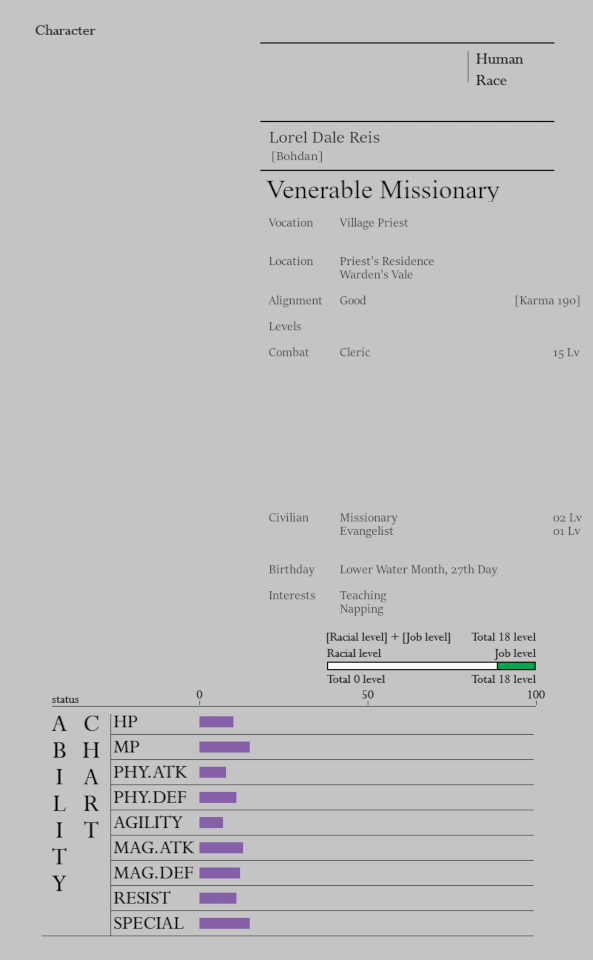
\includegraphics[width=1\linewidth]{images/17LKe7u.png}
    \caption*{Lorel Dale Reis Character Sheet}
\end{figure}

\section*{Character Dossier: Lorel Dale Reis}

Lorel Dale Reis, or Bohdan – as he was known locally to the inhabitants of Warden’s Vale – was born in the southern cities of the Slane Theocracy 119 years before the founding of the Sorcerous Kingdom. The second son of a common warehouse clerk and a seamstress, he was brought up in a meagre household, destined to follow in his father’s footsteps as an apprentice.

 

His fate was changed when a shift occurred in the policies of the Slane Theocracy as its leadership began preparations for the next wave of Players: directing their various institutions to expand recruitment, education and training. Bohdan was swept up as his generation was readied for what may have come. Joining the ranks of the priesthood as an Acolyte, Lorel experienced a curriculum that not only included the Theocracy’s stringent training, but also studied events related to Player waves – notably those of the Eight Greed Kings, the Thirteen Heroes and the Six Great Gods of the Slane Theocracy. The vast majority of this generation never realized what they were being prepared for.

 

Though his tenure as an Acolyte was meant to gird him for those coming times, he ultimately found his calling elsewhere. To the north, the call of a burgeoning Human civilization pulled the young Lorel away from his homeland to answer the growing need for priests and missionaries to both aid the growth of Human realms and spread the faith of the Six Great Gods. At the age of 18, in his search for a place to serve humanity, he encountered Andrei Zahradnik. The intrepid Ranger captured both his admiration and respect, and Lorel would settle in Warden’s Vale, serving the Barony faithfully as its priest for four generations.

 

After receiving news of the Re-Estize's defeat at the Battle of Katze Plains, Bohdan headed the flight of the residents of Warden’s Vale, meaning to lead them to the safety of the Slane Theocracy. He, along with those who followed him, vanished some time later in the wilderness while en route to their destination.